\doublespacing % Do not change - required

\chapter{Results}
\label{ch:results}

%%%%%%%%%%%%%%%%%%%%%%%%%%%%%%%%%%%%%%%
% IMPORTANT
\begin{spacing}{1} %THESE FOUR
\minitoc % LINES MUST APPEAR IN
\end{spacing} % EVERY
\thesisspacing % CHAPTER
% COPY THEM IN ANY NEW CHAPTER
%%%%%%%%%%%%%%%%%%%%%%%%%%%%%%%%%%%%%%%

This chapter reports the results in four parts. First, image-quality metrics act as sanity checks that the translator has not lost basic fidelity (Section~\ref{sec:res_imagequality}), though they are not the main success criterion. Second, downstream metrics across detection, segmentation and embedding spaces ask whether the translated images make frozen RGB-pretrained models behave more like they do on native RGB (Section~\ref{sec:res_downstream}). Third, the teacher ablation study explains how the final recipe was reached, moving from a conventional baseline to the foundation-feature ensemble (Section~\ref{sec:res_ablation}). Finally, the edge section reports the Raspberry~Pi~5 benchmark for the deployed student on both the CPU and the Hailo-8L NPU, and a live on-device demonstration (Section~\ref{sec:res_edge}).

\section{Image Quality}
\label{sec:res_imagequality}

PSNR, SSIM and LPIPS are useful checks that the translator has not lost basic image fidelity, but they are secondary to the downstream behavioural metrics in Section~\ref{sec:res_downstream}. \autoref{tab:res_imagequality} compares raw NIR, the conventional Pix2Pix baseline, the final teacher and the deployment-target student variants. 

\begin{table}[!htbp]
\centering
\scriptsize
\setlength{\tabcolsep}{2.5pt}
\resizebox{\linewidth}{!}{%
\begin{tabular}{lccccc}
\hline
\textbf{Model} & \textbf{PSNR\,(dB), mean [95\% CI]} $\uparrow$ & \textbf{SSIM, mean [95\% CI]} $\uparrow$ & \textbf{LPIPS, mean [95\% CI]} $\downarrow$ & \textbf{Params} & \textbf{Artefact size} \\
\hline
Raw NIR & 16.65 [16.46, 16.84] & 0.656 [0.648, 0.665] & 0.337 [0.330, 0.344] & N/A & N/A \\
Pix2Pix baseline (U-Net) & 24.03 [23.83, 24.24] & 0.752 [0.746, 0.758] & 0.185 [0.180, 0.190] & 54.4\,M & 686.3\,MB checkpoint \\
Teacher (NAFNet-64) & 26.16 [25.91, 26.42] & 0.818 [0.812, 0.824] & 0.103 [0.099, 0.108] & 116\,M & 1{,}425.7\,MB checkpoint \\
Student FP32 (NAFNet-16) & 24.09 [23.86, 24.33] & 0.781 [0.774, 0.787] & 0.146 [0.141, 0.150] & 1.7\,M & 7.1\,MB LiteRT \\
Student mixed-INT8 (NAFNet-16) & 23.57 [23.35, 23.79] & 0.770 [0.763, 0.776] & 0.153 [0.148, 0.158] & 1.7\,M & 2.3\,MB LiteRT \\
\hline
\end{tabular}
}
\caption{Image-quality and artefact-size comparison on the canonical held-out test split. The FP32 student also has a 7.6\,MB ONNX artefact.}
\label{tab:res_imagequality}
\end{table}

The final teacher gives the strongest fidelity result, improving over Pix2Pix by 2.13\,dB PSNR, 0.066 SSIM and 0.082 LPIPS. The width-16 FP32 student trades some of this quality for a $67.3\times$ parameter reduction: relative to the teacher, it loses 2.07\,dB PSNR and 0.037 SSIM, while LPIPS increases by 0.0426. It also matches or beats the Pix2Pix baseline on every pixel and perceptual metric: PSNR ties (24.09 against 24.03), SSIM is higher (0.781 against 0.752) and LPIPS is lower (0.146 against 0.185), all at 1/32 of the parameters. On these traditional metrics the compact student is therefore as good as the GAN baseline, which makes the downstream comparison in Section~\ref{sec:res_downstream} the deciding evidence.

Post-training quantisation introduces a further, measurable quality cost. Relative to the FP32 student, the mixed-INT8 model loses 0.523\,dB PSNR and 0.0114 SSIM, and LPIPS increases by 0.0073. In return, the LiteRT artefact falls from 7.1\,MB to 2.3\,MB. The qualitative examples in \autoref{fig:student_compare_grid} show that the two students preserve the teacher's broad colour and structure on typical cases, while both are somewhat less saturated and detailed than the teacher.

\begin{figure}[!htbp]
\centering
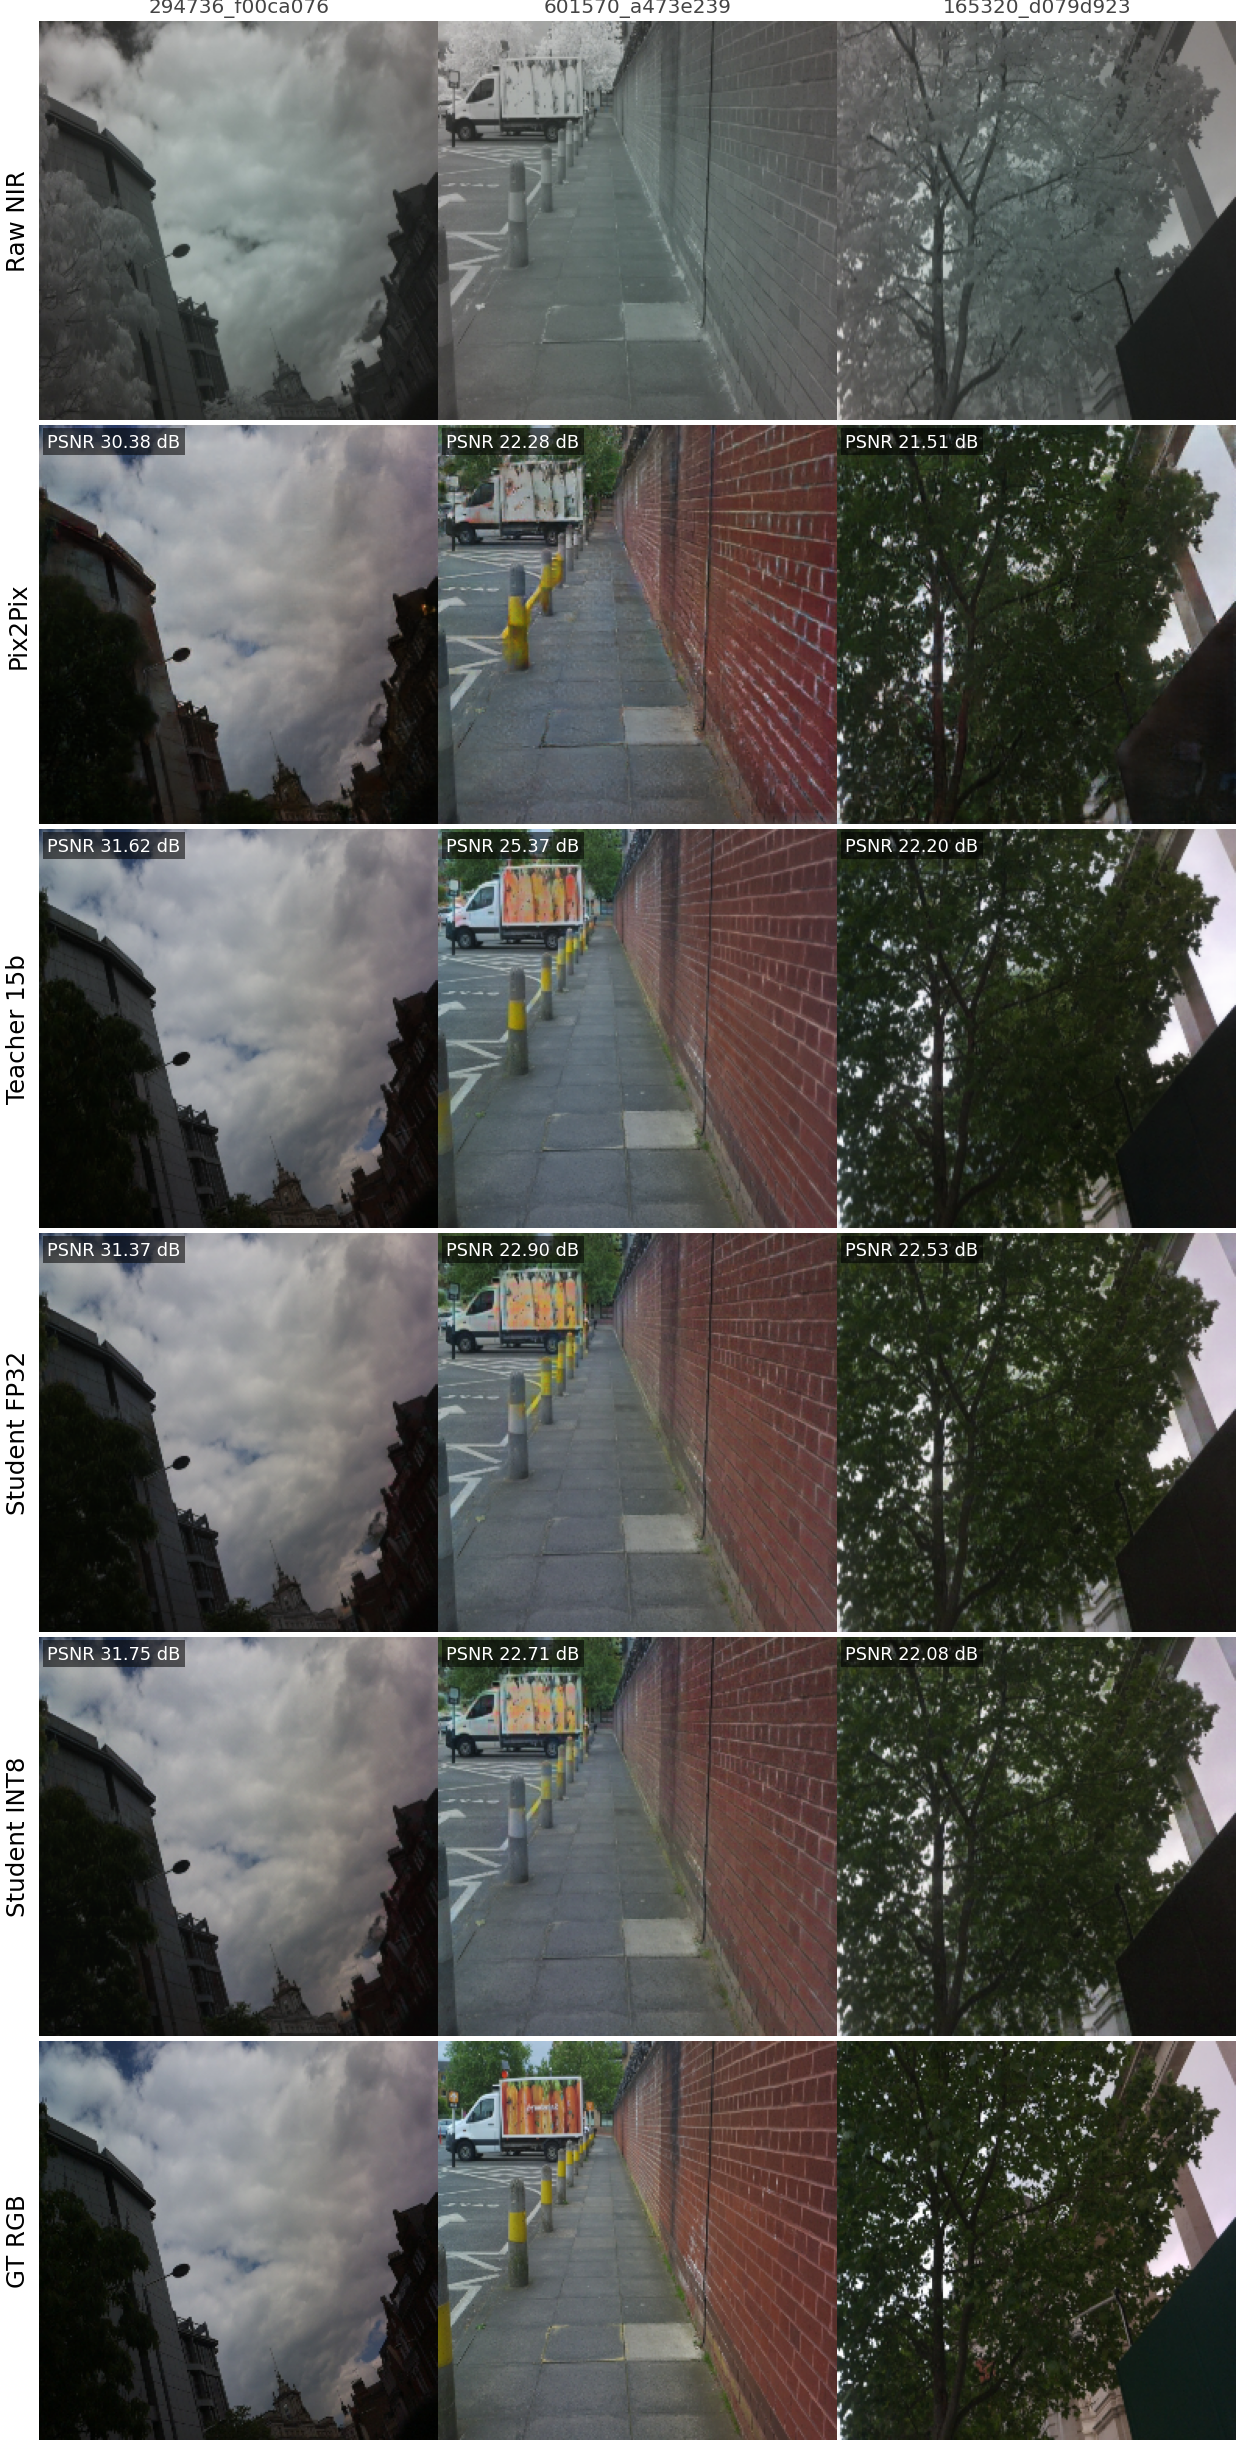
\includegraphics[height=0.9\textheight]{imgs/random_no_people_grid.png}
\caption{Random samples. The rows show, top to bottom: raw NIR, Pix2Pix, teacher, feature-KD student FP32, feature-KD student INT8, and ground-truth RGB. PSNR values are reported for each model.}
\label{fig:student_compare_grid}
\end{figure}

\section{Downstream Agreement}
\label{sec:res_downstream}

The final teacher, FP32 student and deployed mixed-INT8 student are evaluated with a panel of frozen RGB-pretrained models, asking whether translation restores behaviour closer to that observed on native RGB without retraining. The evaluation covers foundation-model embeddings, object detection, semantic segmentation and depth estimation. These are behavioural-agreement measurements against native-RGB model outputs rather than human-labelled task accuracy.

\subsection{Foundation and Independent Embedding Agreement}

\autoref{tab:res_pixel_embedding} measures cosine agreement with native RGB in four representation spaces. DINOv2-S supplied a training loss, and the CLIP evaluator is partially related to training because CLIP-B/32 supplied a loss and checkpoint-selection signal while the test evaluator uses CLIP-B/16. DINOv2-L~\cite{oquab2024dinov2} and SigLIP2~\cite{tschannen2025siglip2} did not appear in the training objective and therefore provide the stronger independent probes. CLIP-FID complements the per-image cosine metrics with a distribution-level comparison over the complete test split.

\begin{table}[!htbp]
\centering
\scriptsize
\setlength{\tabcolsep}{2.5pt}
\resizebox{\linewidth}{!}{%
\begin{tabular}{llcccccc}
\hline
\textbf{Evaluator} & \textbf{Training overlap} & \textbf{Raw NIR} & \textbf{Pix2Pix} & \textbf{Teacher} & \textbf{Student FP32} & \textbf{Student INT8} \\
\hline
\multicolumn{7}{l}{\textbf{Cosine similarity, mean [95\% CI]} $\uparrow$} \\
DINOv2-S & Yes & 0.7273 [0.7185, 0.7361] & 0.8072 [0.8005, 0.8136] & 0.9499 [0.9465, 0.9530] & 0.9228 [0.9188, 0.9266] & 0.9166 [0.9124, 0.9206] \\
DINOv2-L & No & 0.7282 [0.7198, 0.7365] & 0.7229 [0.7153, 0.7304] & 0.9206 [0.9162, 0.9248] & 0.8816 [0.8765, 0.8864] & 0.8709 [0.8654, 0.8761] \\
CLIP-B/16 & Partial & 0.8563 [0.8534, 0.8593] & 0.8774 [0.8739, 0.8809] & 0.9572 [0.9550, 0.9593] & 0.9287 [0.9259, 0.9315] & 0.9202 [0.9173, 0.9230] \\
SigLIP2 base/256 & No & 0.8829 [0.8803, 0.8854] & 0.8940 [0.8909, 0.8971] & 0.9619 [0.9600, 0.9636] & 0.9459 [0.9437, 0.9480] & 0.9427 [0.9404, 0.9449] \\
\hline
\multicolumn{7}{l}{\textbf{Distribution-level distance} $\downarrow$} \\
CLIP-FID & Partial & 17.86 & 11.94 & 2.47 & 5.50 & 6.95 \\
\hline
\end{tabular}
}
\caption{Embedding agreement with native RGB. Cosine rows report per-image means with 95\% image-bootstrap confidence intervals. ``Partial'' shows evaluator-family overlap rather than reuse of the exact test-time weights.}
\label{tab:res_pixel_embedding}
\end{table}

The teacher is strongest on every representation metric, but the students retain substantial improvement over raw NIR. On the independent DINOv2-L probe, cosine similarity rises from 0.7282 for raw NIR to 0.8816 for the FP32 student and 0.8709 after quantisation, corresponding to gap closures of 0.566 and 0.525. On independent SigLIP2, the respective closures are 0.538 and 0.511. The Pix2Pix baseline closes almost none of this representation gap, with closures of -0.020 on DINOv2-L and +0.095 on SigLIP2. The confidence intervals for raw NIR and both student variants are clearly separated on both independent probes.

Quantisation reduces every cosine score slightly, with DINOv2-L falling by 0.0107 and SigLIP2 by 0.0032 relative to the FP32 student. The distribution-level effect is larger, with CLIP-FID increasing from 5.50 to 6.95, a 26.37\% deterioration, although it remains substantially below the raw-NIR value of 17.86. These results support retained representation-level agreement after compression and quantisation, but DINOv2-S and CLIP-family scores are treated as supporting rather than independent evidence because of their relationship to the training objective.

\subsection{Object Detection}

Detection agreement is evaluated with YOLOv8m and RT-DETR-L using COCO-style mAP at IoU 0.5 and over thresholds 0.5:0.95. Native-RGB detections are treated as pseudo-ground truth, so native-RGB self-agreement is 1 by definition.

\begin{table}[!htbp]
\centering
\footnotesize
\begin{tabular}{llccccc}
\hline
\textbf{Detector} & \textbf{Metric} & \textbf{Raw NIR} & \textbf{Pix2Pix} & \textbf{Teacher} & \textbf{Student FP32} & \textbf{Student INT8} \\
\hline
YOLOv8m & mAP@0.5 $\uparrow$ & 0.224 & 0.106 & 0.308 & 0.284 & 0.288 \\
        & mAP@0.5:0.95 $\uparrow$ & 0.187 & 0.081 & 0.259 & 0.242 & 0.246 \\
RT-DETR-L & mAP@0.5 $\uparrow$ & 0.243 & 0.148 & 0.390 & 0.297 & 0.283 \\
          & mAP@0.5:0.95 $\uparrow$ & 0.205 & 0.120 & 0.339 & 0.252 & 0.241 \\
\hline
\end{tabular}
\caption{Object-detection agreement with native-RGB pseudo-labels. Metrics use COCO-style mAP@0.5 and mAP@0.5:0.95. Reference detections come from the same frozen detector on native RGB rather than human annotations.}
\label{tab:res_detection}
\end{table}

The teacher improves both metrics for both detectors and produces the strongest detection agreement overall. Using the primary mAP@0.5 metric, its gap closure is 0.108 for YOLOv8m and 0.194 for RT-DETR-L. Distillation reduces these gains, and the FP32 student's closures are 0.077 and 0.072 respectively. Nevertheless, both remain positive, showing that the selected student moves both detector outputs toward their native-RGB behaviour rather than merely preserving the raw-NIR baseline. Pix2Pix, by contrast, falls below the raw-NIR baseline on both detectors, with mAP@0.5 closures of -0.152 for YOLOv8m and -0.125 for RT-DETR-L.

Quantisation has a detector-dependent effect. YOLOv8m mAP@0.5 rises slightly from 0.284 to 0.288, increasing gap closure from 0.077 to 0.083. RT-DETR-L mAP@0.5 falls from 0.297 to 0.283, reducing closure from 0.072 to 0.053. The same direction is visible in mAP@0.5:0.95. Thus, INT8 retains positive agreement recovery for both independent detectors, but the small YOLO improvement should not be interpreted as a general benefit of quantisation.

\subsection{Semantic Segmentation}
\label{sec:res_seg}

Segmentation is evaluated using Dice agreement with the native-RGB SegFormer prediction on images where the reference class occupies at least 5\% of pixels. ADE20K and Cityscapes are reported separately because their category sets and training distributions differ.

\autoref{tab:res_seg_ade} reports the four ADE20K classes used in the primary summary. \autoref{tab:res_seg_cityscapes} reports the 18 defined Cityscapes classes. Traffic light has no qualifying examples and is excluded from the class-unweighted mean.

\begin{table}[!htbp]
\centering
\scriptsize
\setlength{\tabcolsep}{2.5pt}
\resizebox{\linewidth}{!}{%
\begin{tabular}{lcccccc}
\hline
\textbf{Class} & \textbf{$n$} & \textbf{Raw NIR [95\% CI]} & \textbf{Pix2Pix [95\% CI]} & \textbf{Teacher [95\% CI]} & \textbf{Student FP32 [95\% CI]} & \textbf{Student INT8 [95\% CI]} \\
\hline
Tree & 665 & 0.625 [0.598, 0.651] & 0.897 [0.885, 0.908] & 0.945 [0.938, 0.951] & 0.921 [0.912, 0.930] & 0.917 [0.908, 0.926] \\
Person & 226 & 0.685 [0.643, 0.724] & 0.679 [0.642, 0.714] & 0.856 [0.831, 0.879] & 0.834 [0.810, 0.857] & 0.823 [0.797, 0.847] \\
Building & 869 & 0.797 [0.781, 0.811] & 0.862 [0.851, 0.874] & 0.915 [0.905, 0.924] & 0.894 [0.883, 0.904] & 0.891 [0.879, 0.901] \\
Road & 323 & 0.669 [0.636, 0.701] & 0.762 [0.733, 0.789] & 0.881 [0.864, 0.899] & 0.845 [0.824, 0.865] & 0.842 [0.821, 0.861] \\
\hline
Class-unweighted mean & -- & 0.694 & 0.750 & 0.899 & 0.874 & 0.868 \\
\hline
\end{tabular}
}
\caption{SegFormer-B0-ADE20K Dice agreement with native-RGB pseudo-labels. Rows include only test images where the native-RGB reference class covers at least 5\% of pixels.}
\label{tab:res_seg_ade}
\end{table}

\begin{table}[!htbp]
\centering
\scriptsize
\setlength{\tabcolsep}{2pt}
\resizebox{\linewidth}{!}{%
\begin{tabular}{lcccccc}
\hline
\textbf{Class} & \textbf{$n$} & \textbf{Raw NIR [95\% CI]} & \textbf{Pix2Pix [95\% CI]} & \textbf{Teacher [95\% CI]} & \textbf{Student FP32 [95\% CI]} & \textbf{Student INT8 [95\% CI]} \\
\hline
Road & 680 & 0.653 [0.627, 0.678] & 0.789 [0.770, 0.809] & 0.846 [0.830, 0.861] & 0.811 [0.794, 0.828] & 0.811 [0.793, 0.828] \\
Sidewalk & 321 & 0.528 [0.494, 0.561] & 0.566 [0.533, 0.599] & 0.743 [0.719, 0.767] & 0.661 [0.631, 0.690] & 0.635 [0.603, 0.666] \\
Building & 920 & 0.700 [0.684, 0.716] & 0.805 [0.792, 0.817] & 0.864 [0.852, 0.876] & 0.833 [0.820, 0.846] & 0.822 [0.808, 0.836] \\
Wall & 109 & 0.263 [0.209, 0.316] & 0.407 [0.345, 0.472] & 0.618 [0.560, 0.670] & 0.539 [0.481, 0.594] & 0.525 [0.471, 0.577] \\
Fence & 184 & 0.489 [0.440, 0.538] & 0.500 [0.456, 0.544] & 0.692 [0.651, 0.731] & 0.618 [0.573, 0.660] & 0.609 [0.565, 0.652] \\
Pole & 32 & 0.679 [0.581, 0.766] & 0.627 [0.522, 0.723] & 0.747 [0.636, 0.843] & 0.717 [0.630, 0.790] & 0.632 [0.512, 0.742] \\
Traffic sign & 4 & 0.211 [0.000, 0.610] & 0.159 [0.000, 0.414] & 0.418 [0.064, 0.772] & 0.398 [0.000, 0.796] & 0.410 [0.000, 0.821] \\
Vegetation & 808 & 0.641 [0.618, 0.664] & 0.878 [0.867, 0.887] & 0.934 [0.927, 0.941] & 0.910 [0.901, 0.919] & 0.903 [0.893, 0.911] \\
Terrain & 86 & 0.041 [0.020, 0.066] & 0.864 [0.812, 0.908] & 0.881 [0.833, 0.924] & 0.856 [0.801, 0.903] & 0.857 [0.805, 0.902] \\
Sky & 542 & 0.767 [0.740, 0.792] & 0.921 [0.907, 0.935] & 0.957 [0.947, 0.966] & 0.939 [0.927, 0.951] & 0.920 [0.904, 0.936] \\
Person & 271 & 0.601 [0.563, 0.639] & 0.619 [0.584, 0.653] & 0.775 [0.745, 0.805] & 0.725 [0.691, 0.758] & 0.714 [0.680, 0.748] \\
Rider & 32 & 0.091 [0.023, 0.176] & 0.402 [0.317, 0.488] & 0.702 [0.628, 0.764] & 0.591 [0.500, 0.671] & 0.479 [0.377, 0.577] \\
Car & 191 & 0.683 [0.639, 0.726] & 0.634 [0.587, 0.680] & 0.793 [0.756, 0.828] & 0.726 [0.682, 0.768] & 0.712 [0.667, 0.755] \\
Truck & 31 & 0.296 [0.193, 0.405] & 0.223 [0.127, 0.330] & 0.422 [0.304, 0.543] & 0.351 [0.245, 0.465] & 0.300 [0.190, 0.421] \\
Bus & 16 & 0.334 [0.169, 0.509] & 0.410 [0.268, 0.552] & 0.478 [0.294, 0.662] & 0.401 [0.226, 0.581] & 0.361 [0.183, 0.545] \\
Train & 31 & 0.195 [0.112, 0.284] & 0.115 [0.042, 0.206] & 0.349 [0.245, 0.453] & 0.198 [0.107, 0.301] & 0.163 [0.082, 0.259] \\
Motorcycle & 18 & 0.303 [0.172, 0.452] & 0.482 [0.357, 0.605] & 0.726 [0.620, 0.820] & 0.612 [0.535, 0.695] & 0.641 [0.574, 0.717] \\
Bicycle & 36 & 0.580 [0.472, 0.684] & 0.721 [0.651, 0.786] & 0.716 [0.624, 0.803] & 0.666 [0.572, 0.757] & 0.655 [0.557, 0.751] \\
\hline
Mean excluding traffic light & -- & 0.447 & 0.572 & 0.703 & 0.642 & 0.619 \\
\hline
\end{tabular}
}
\caption{SegFormer-B0-Cityscapes Dice agreement with native-RGB pseudo-labels. Traffic light has no qualifying examples and is excluded from the mean. All reported values include 95\% bootstrap confidence intervals from 10{,}000 image-level resamples.}
\label{tab:res_seg_cityscapes}
\end{table}

Both segmentation tasks show a larger recovery than detection. ADE20K class-mean Dice improves from 0.694 on raw NIR to 0.874 for the FP32 student and 0.868 after INT8 conversion, giving gap closures of 0.587 and 0.569. Cityscapes class-mean Dice improves from 0.447 to 0.642 for FP32 and 0.619 for INT8, giving closures of 0.351 and 0.311. Pix2Pix achieves smaller but positive closures of +0.183 on ADE20K and +0.226 on Cityscapes, making segmentation the one task family where the baseline recovers some native-RGB behaviour. Quantisation slightly reduces both means, with the larger loss on the Cityscapes distribution.

\subsection{Depth}

Depth agreement is evaluated with DepthAnything-Small. The metric is per-image min--max-normalised L1 distance to the native-RGB depth prediction, so lower is better.

\begin{table}[!htbp]
\centering
\footnotesize
\resizebox{\linewidth}{!}{%
\begin{tabular}{llccccc}
\hline
\textbf{Model} & \textbf{Metric} & \textbf{Raw NIR} & \textbf{Pix2Pix} & \textbf{Teacher} & \textbf{Student FP32} & \textbf{Student INT8} \\
\hline
DepthAnything-Small & Normalised L1 $\downarrow$ & 0.677 [0.641, 0.715] & 0.678 [0.642, 0.715] & 0.365 [0.344, 0.387] & 0.424 [0.402, 0.447] & 0.455 [0.429, 0.482] \\
\hline
\end{tabular}
}
\caption{DepthAnything-Small agreement with native-RGB depth predictions. Normalised L1 is computed after per-image min--max normalisation and should not be read as metres.}
\label{tab:res_depth}
\end{table}

The FP32 and INT8 students both improve substantially over raw NIR. Their normalised L1 closures are 0.374 and 0.328 respectively. Pix2Pix's closure is -0.001, so its depth agreement is indistinguishable from raw NIR. Quantisation increases the error by 0.0308 relative to the FP32 student, which is the largest relative quality loss among the five primary tasks.

\subsection{Headline Gap-Closure Summary}
\label{sec:res_gapclosure}

\autoref{tab:res_gapclosure} summarises the primary success criterion. The five primary tasks are the two detection models, the two segmentation distributions and the depth evaluator. Independent embedding probes are shown as supporting evidence because they are useful checks on representation recovery but are not counted as separate primary tasks.

\begin{table}[!htbp]
\centering
\footnotesize
\resizebox{\linewidth}{!}{%
\begin{tabular}{llccccccc}
\hline
\textbf{Task} & \textbf{Primary metric} & \textbf{Raw} & \textbf{Pix2Pix} & \textbf{Pix2Pix closure} & \textbf{Student FP32} & \textbf{FP32 closure} & \textbf{Student INT8} & \textbf{INT8 closure} \\
\hline
Detection 1 & YOLOv8m mAP@0.5 & 0.224 & 0.106 & -0.152 & 0.284 & +0.077 & 0.288 & +0.083 \\
Detection 2 & RT-DETR-L mAP@0.5 & 0.243 & 0.148 & -0.125 & 0.297 & +0.072 & 0.283 & +0.053 \\
Segmentation 1 & ADE class-mean Dice & 0.694 & 0.750 & +0.183 & 0.874 & +0.587 & 0.868 & +0.569 \\
Segmentation 2 & Cityscapes class-mean Dice & 0.447 & 0.572 & +0.226 & 0.642 & +0.351 & 0.619 & +0.311 \\
Depth & Normalised L1 & 0.677 & 0.678 & -0.001 & 0.424 & +0.374 & 0.455 & +0.328 \\
Independent embedding & DINOv2-L cosine & 0.728 & 0.723 & -0.020 & 0.882 & +0.566 & 0.871 & +0.525 \\
Independent embedding & SigLIP2 cosine & 0.883 & 0.894 & +0.095 & 0.946 & +0.538 & 0.943 & +0.511 \\
\hline
\end{tabular}
}
\caption{Headline gap-closure summary for the selected student before and after mixed-INT8 export. Positive closure means the translated output is closer to native-RGB model behaviour than raw NIR. For the lower-is-better depth metric, the closure sign is inverted by the harness. }
\label{tab:res_gapclosure}
\end{table}

Both student precisions pass S2 with positive closure on all five primary tasks, and neither falls below its raw-NIR baseline. Quantisation retains positive closure on all seven reported probes, although it reduces six of the seven closure values. YOLOv8m is the exception and improves slightly.

Pix2Pix is the standard baseline for paired image-to-image translation and the formulation most later methods build on~\cite{isola2017image,wang2018pix2pixhd,park2019spade,pix2next2024}, so it is a fair point of comparison. It is also the sharpest illustration of why downstream agreement, not pixel fidelity, is the right success criterion. It ties the student on pixel and structural fidelity, yet on the independent DINOv2-L probe it sits at 0.723, indistinguishable from the 0.728 of doing no translation at all, and on depth its 0.678 equals raw NIR exactly. The student reaches 0.882 and 0.424 on the same probes. On detection Pix2Pix is worse than the untranslated input, falling from raw NIR's 0.224 to 0.106 mAP@0.5 on YOLOv8m and from 0.243 to 0.148 on RT-DETR-L, closures of -0.152 and -0.125, where both student precisions stay positive. A baseline that looks competitive on classic metrics therefore contributes almost nothing to the downstream behaviour the translator is meant to restore. It is also a 54.4\,M-parameter model against the student's 1.7\,M, so unlike the student it is not a candidate for the Raspberry~Pi.

\section{Teacher Ablation Study}
\label{sec:res_ablation}

\subsection{Ablation Results}

\autoref{tab:abl_summary} reports ablation evidence for the teacher recipe. All NAFNet variants outperform Pix2Pix on PSNR, LPIPS, DINOv2-L, ADE Dice and depth L1. Removing the foundation-feature ensemble (No FM) improves pixel fidelity but markedly reduces downstream agreement metrics, indicating that the feature-matching term is essential to the downstream gains. The other ablations (No GAN, No MS-SSIM, No FM warm-up) sit within confidence intervals on DINOv2-L and depth, suggesting these components are not individually critical on those probes. The adversarial term nevertheless earns its place on detection: removing it drops YOLO closure from +0.108 to +0.077, the largest detection change among these ablations, and at weight 0.3 it adds little training cost or instability. The final teacher therefore retains the full objective and represents the clean baseline for deployment.

\begin{table}[!htbp]
\centering
\scriptsize
\setlength{\tabcolsep}{2pt}
\resizebox{\linewidth}{!}{%
\begin{tabular}{lp{0.24\linewidth}cccccc}
\hline
\textbf{Configuration} & \textbf{Exact change} & \textbf{PSNR} & \textbf{LPIPS} & \textbf{DINOv2-L} & \textbf{YOLO closure} & \textbf{ADE closure} & \textbf{Depth L1} \\
\hline
Raw NIR & no translation & 16.65 & 0.337 & 0.728 & 0.000 & 0.000 & 0.677 \\
Pix2Pix & U-Net baseline & 24.03 & 0.185 & 0.723 & -0.152 & 0.183 & 0.678 \\
No FM & FM weights zero & 27.10 & 0.098 & 0.886 & +0.011 & 0.619 & 0.420 \\
No GAN & GAN disabled & 26.33 & 0.100 & 0.923 & +0.077 & 0.667 & 0.347 \\
No MS-SSIM & MS-SSIM disabled & 26.29 & 0.102 & 0.922 & +0.076 & 0.653 & 0.348 \\
No FM warm-up& FM active without warm-up & 26.31 & 0.101 & 0.921 & +0.064 & 0.665 & 0.353 \\
Final teacher & full objective & 26.16 & 0.103 & 0.921 & +0.108 & 0.670 & 0.365 \\
\hline
\end{tabular}
}
\caption{Teacher ablation summary on the canonical held-out test split.}
\label{tab:abl_summary}
\end{table}



\subsection{Pixel-side versus feature-side changes}
\label{sec:res_abl_lossfixes}

Two intermediate objective changes preceded the final ensemble. The first targeted the pixel side, using an NIR-gradient-weighted L1 that downweights the loss in flat NIR regions, on the reasoning that colour is poorly determined there and penalising those regions equally pushes the model toward desaturated, average colour. In practice this made almost no difference, and if anything cost a small amount of performance, indicating that the baseline's weakness was not a mis-weighted pixel term. The change that mattered was on the feature side, adding a \emph{task-facing feature loss} in which the generated and real RGB are passed through frozen RGB-trained models and the differences in their early and mid activations are penalised. This directly optimises agreement in the representations the downstream panel uses, rather than pixel colour or a generic VGG perceptual space. The first feature-supervised NAFNet used ResNet-50 and SegFormer features, providing the proof of concept that led to the foundation-model ensemble of the final teacher.

\begin{figure}[!htbp]
\centering
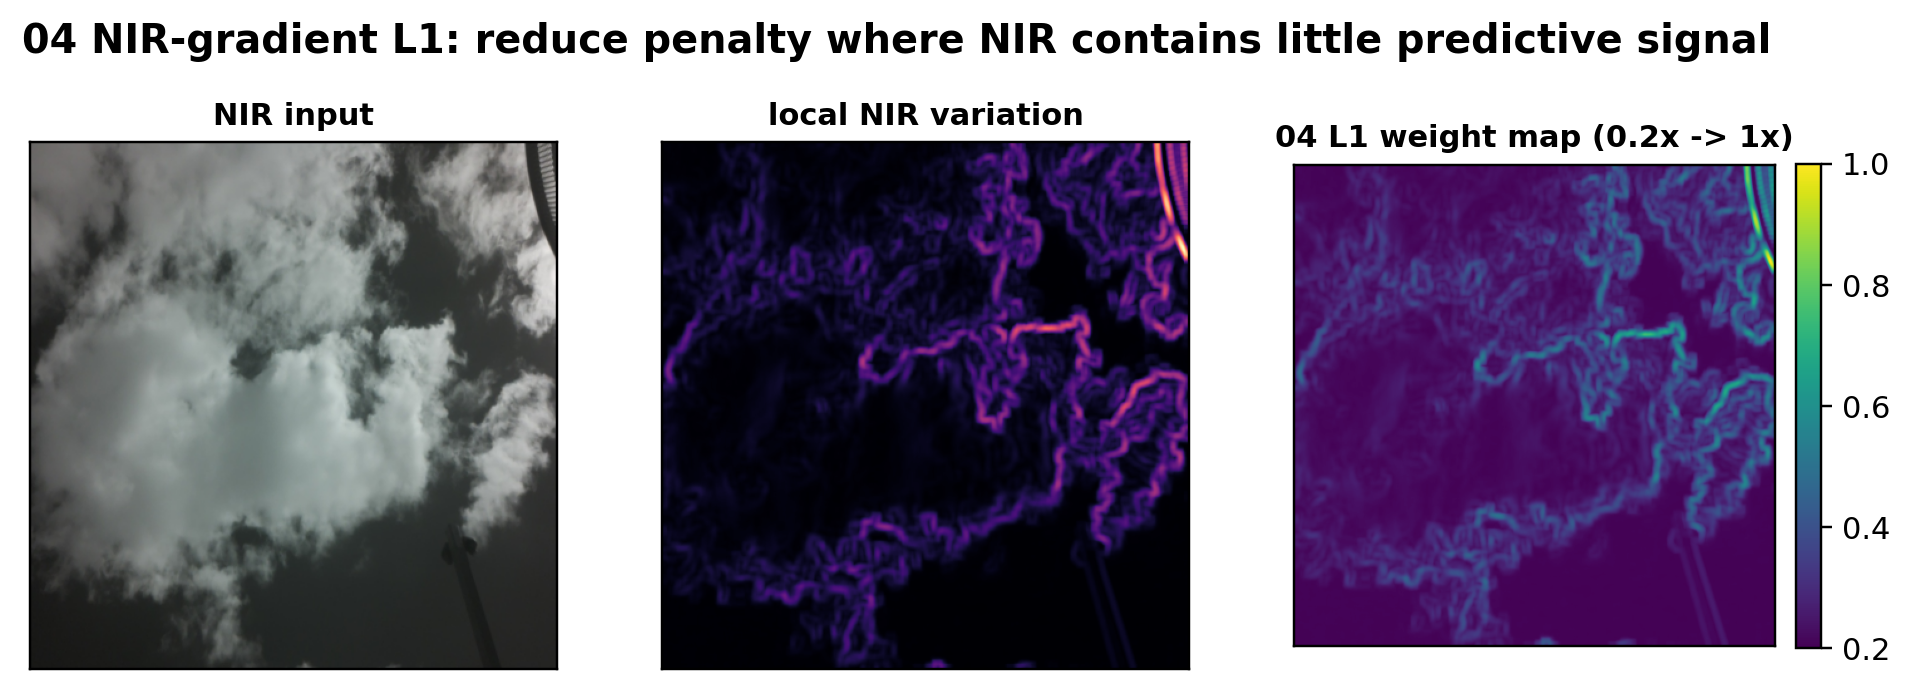
\includegraphics[width=\linewidth]{imgs/ablations/nir_gradient_l1.png}
\caption{NIR-gradient-weighted L1. From the NIR input (left), local NIR variation (centre) drives a per-pixel L1 weight map (right) that scales the penalty from $0.2\times$ in flat, low-signal regions to $1\times$ at strong NIR edges. In practice this reweighting made almost no difference to downstream agreement, indicating the baseline's weakness was not a mis-weighted pixel term.}
\label{fig:nir_gradient_l1}
\end{figure}

\section{Student Distillation Ablations}
\label{sec:res_student_ablation}

The teacher ablations above choose the high-capacity teacher. A separate question is how to compress it into the width-16 student without losing the downstream behaviour that made the teacher useful. These are not different student architectures: each variant uses the same NAFNet-16 backbone and the same teacher-output L1 distillation term. What changes is the auxiliary supervision used to teach the small model what matters.

\begin{description}
    \item[Baseline KD.] This is the minimum task-facing student. It distils the teacher output with an L1 term and adds DINOv2 and CLIP feature losses against the RGB ground truth. It tests whether the compact student can recover the teacher's broad semantic alignment using only generic foundation-feature supervision.
    \item[Downstream heads.] This keeps the same student architecture but broadens the feature losses to include ResNet-50, SegFormer and DepthAnything. It tests whether adding classifier, segmentation and depth representations preserves the downstream behaviours measured by the evaluation harness, rather than only matching generic image embeddings.
    \item[Feature KD.] This adds feature-level knowledge distillation from the teacher: frozen-feature activations are matched between the student's output and the teacher's output, not only between the student's output and RGB ground truth. It tests whether the student should imitate the teacher's representation-space behaviour directly when the teacher's output is the deployed target.
\end{description}

\autoref{tab:student_distill_ablation} compares these student-training variants.

\begin{table}[!htbp]
\centering
\footnotesize
\setlength{\tabcolsep}{3pt}
\resizebox{\linewidth}{!}{%
\begin{tabular}{lp{0.28\linewidth}cccccccc}
\hline
\textbf{Student variant} & \textbf{Additional signal} & \textbf{PSNR} & \textbf{LPIPS} & \textbf{CLIP-B/16} & \textbf{DINOv2-L} & \textbf{ADE mean} & \textbf{City mean} & \textbf{YOLO} & \textbf{RT-DETR} \\
\hline
Baseline KD & DINOv2 and CLIP to RGB GT & 24.08 & 0.152 & 0.923 & 0.875 & 0.863 & 0.631 & 0.264 & 0.296 \\
Downstream heads & DINOv2, CLIP, ResNet-50, SegFormer and DepthAnything & 23.59 & 0.155 & 0.917 & 0.867 & 0.860 & 0.624 & 0.220 & 0.302 \\
Feature KD & downstream heads plus feature match to teacher output & \textbf{24.09} & \textbf{0.146} & \textbf{0.929} & \textbf{0.882} & \textbf{0.874} & \textbf{0.642} & \textbf{0.284} & 0.297 \\
\hline
\end{tabular}
}
\caption{Student distillation ablation for the width-16 NAFNet. All variants use 1.7\,M parameters and the same backbone, and only the auxiliary supervision differs. YOLO and RT-DETR columns report mAP@0.5 agreement.}
\label{tab:student_distill_ablation}
\end{table}

The feature-KD student is selected by the predeclared highest validation CLIP-cosine rule and is also strongest on most of the quality and downstream probes. It compresses the 116\,M teacher parameters to 1.7\,M, a $67.3\times$ reduction, while losing 2.07\,dB PSNR and 0.039 DINOv2-L cosine relative to the teacher.

\section{Generalisation to Other Modalities}
\label{sec:res_modality_extension}

The foundation-model feature-matching recipe is not specific to NIR, so it was also tested on thermal and SAR imagery to find where it stops working.

On thermal imagery (KAIST), which shares no spectral overlap with the visible band, the recipe transfers without modification. CLIP cosine similarity reaches 0.924 compared to 0.46 on raw thermal, and static scene classes improve in downstream segmentation (roads +0.3 Dice, vegetation +0.7 Dice, sky +0.8 Dice). The person class fails, because raw thermal's strong pedestrian contrast (people are warm) is lost when the model spends capacity on global colour synthesis. The same weakness appears in the NIR results.

\begin{figure}[!htbp]
\centering
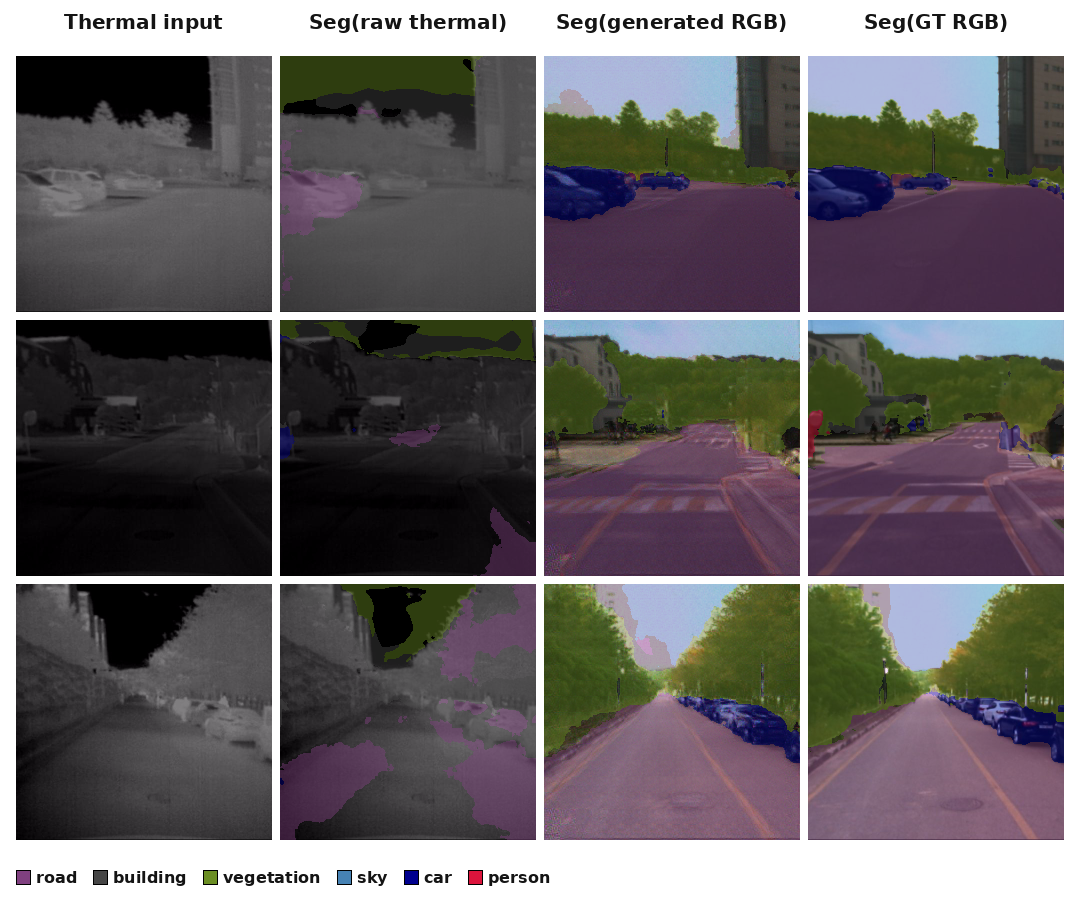
\includegraphics[width=0.90\linewidth]{imgs/seg_kaist.png}
\caption{Downstream segmentation improvement on KAIST thermal. Structures like roads, vegetation and buildings become detectable in the translated output where raw thermal leaves them invisible to standard segmentation models.}
\label{fig:kaist_seg}
\end{figure}

SAR (WHU-SAR-VV, paired SAR/optical patches derived from the WHU-OPT-SAR dataset~\cite{li2022whuoptsar}) is where the approach breaks down. Pixel metrics collapse (PSNR 13.3, SSIM 0.121) and the model plateaus early, while downstream gains are marginal, with EuroSAT~\cite{helber2019eurosat} classification improving from 0.165 to 0.425 and RemoteCLIP~\cite{liu2024remoteclip} cosine reaching 0.759. The recipe helps rare classes (tree Dice improves 10$\times$ from near-invisibility) but absolute performance remains low. The plateau suggests that speckle-aware losses, SAR-specific pretraining or dedicated SAR encoders would be needed to close the gap further.

\section{Edge Performance}
\label{sec:res_edge}
\label{sec:pi_deployment}

For deployment the 116\,M-parameter teacher is distilled into the compact width-16 student selected in Section~\ref{sec:res_student_ablation}. The student was benchmarked on the Raspberry~Pi~5, on the CPU through LiteRT with XNNPACK and ONNX Runtime, and on the Hailo-8L NPU on the Pi AI HAT+. The device ran Raspberry Pi OS on kernel 6.12.75 with HailoRT and Hailo firmware 4.23.0. CPU testing used 100 real test images at $256\times256$ and batch size one, with 10 warmup iterations followed by 100 measurement runs on the default 4-thread configuration. All CPU figures are model-inference latency, the runtime's invoke call on an already prepared input tensor, excluding image decode and pre- and post-processing, while NPU figures are Hailo-8L hardware latency. \autoref{tab:res_edge} reports the results, together with the larger width-32 student variant (11.6\,M parameters, configuration in \autoref{tab:student_arch}) that was also compiled for the NPU.

\begin{table}[!htbp]
\centering
\footnotesize
\begin{tabular}{llccc}
\hline
\textbf{Backend} & \textbf{Model} & \textbf{Latency (ms)} & \textbf{FPS} & \textbf{Artefact} \\
\hline
Hailo-8L NPU & Width-16 student & 36.3 & 27.2 & 17.7\,MB HEF \\
Hailo-8L NPU & Width-32 student & 91.5 & 10.8 & 50.4\,MB HEF \\
CPU LiteRT INT8 & Width-16 student & 198.0 & 5.05 & 2.3\,MB \\
CPU LiteRT FP32 & Width-16 student & 227.2 & 4.40 & 7.1\,MB \\
CPU LiteRT INT8 & Width-32 student & 517.0 & 1.93 & 13.0\,MB \\
CPU ONNX FP32 & Width-16 student & 225.2 & 4.44 & 7.6\,MB \\
CPU ONNX INT8 & Width-16 student & 372.8 & 2.68 & 2.5\,MB \\
\hline
\end{tabular}
\caption{Raspberry~Pi~5 benchmark. CPU rows are model-inference latency at four threads (LiteRT through XNNPACK; ONNX rows from a separate session on the same device, input size and thread configuration), and NPU rows are Hailo-8L hardware latency. The width-16 LiteRT mixed-INT8 student is the selected deployment model; it meets the 5\,FPS target on the CPU and clears it with a wide margin on the NPU.}
\label{tab:res_edge}
\end{table}

\paragraph{Throughput and latency.}
On the CPU, only the mixed-INT8 LiteRT student meets the 5\,FPS target, at 5.05\,FPS (p95: 221.2\,ms) against the FP32 student's 4.40\,FPS (p95: 242.1\,ms). The 15\% throughput gain from quantisation runs contrary to the expectation that compressed models trade latency for size. It reflects the narrower operator set of INT8 kernels and the reduced memory bandwidth required, and it makes the INT8 export not merely smaller but necessary to reach the target at all. The margin is nevertheless slim. INT8 latency varied between 180.1 and 252.5\,ms across the 100 timed runs, consistent with normal scheduler and frequency-governor variation under sustained four-thread load, so the mean meets the 200\,ms budget but the 95th percentile does not, and the CPU path should be regarded as marginal against N1. The Hailo NPU removes this concern, running the same student at 27.2\,FPS, a $5.4\times$ speed-up, and lifting the width-32 student from 1.9\,FPS on the CPU to 10.8\,FPS.

\paragraph{LiteRT vs ONNX.}
The ONNX FP32 export is comparable to LiteRT in size and latency (\autoref{tab:res_edge}), but the quantised path is decisive. ONNX INT8 runs at 2.68\,FPS, far short of the target even allowing for session-to-session variation, where LiteRT INT8 reaches 5.05\,FPS. LiteRT is therefore the deployment runtime, with the ONNX exports retained only for cross-platform portability.

\paragraph{Memory footprint.}
The mixed-INT8 artefact is 2.3\,MB against 7.1\,MB for FP32, a $3.1\times$ reduction coming almost entirely from weight quantisation. Peak memory during sustained inference was under 50\,MB, dominated by input/output buffers and the activation cache rather than model parameters, against 7.6\,GB of RAM available on the idle device, and swap (2.0\,GB configured) was never touched.

\paragraph{Sustained operation and thermal behaviour.}
Sustained operation was checked with a sixty-second continuous NPU run of the selected student. Throughput held at 27.3\,FPS across the full run with no degradation, the Pi temperature rose from 59.8 to 64.8\,\textdegree C, and the throttle status stayed clear for every one-second sample, so there was no under-voltage or frequency cap. On-chip Hailo power telemetry is not exposed on the Pi AI HAT+, so power is reported through the Pi-level thermal evidence rather than a board sensor.

\paragraph{Requirement decisions.}
Both N1 and N2 are met. The selected student clears the 5\,FPS throughput target on both the CPU and the NPU, and the 2.3\,MB artefact and sub-50\,MB peak memory run without swap, out-of-memory failure or thermal throttling, so the edge-deployment objective is verified on the target device. Because the CPU margin is slim, with the p95 latency above the 200\,ms budget, the Hailo-8L path is the recommended backend where headroom for pre-processing or tighter tail latency is required.

\subsection{Live demonstration}
\label{sec:res_live_demo}

A real-time web application runs the full pipeline on the Pi and serves it over the network (\autoref{fig:webapp_live}). It captures NIR frames from the rig camera, translates them with the student, and segments the NIR input, the generated RGB and a live RGB reference from a second camera with a frozen SegFormer-B0 Cityscapes model, displaying all three side by side. The translator backend is switchable at runtime between the two Hailo HEFs and four CPU LiteRT profiles, which lets the CPU and NPU paths be compared live. The image-quality numbers are computed against the second camera under a single global homography, which is not pixel-perfect, and are live single-frame measurements that vary with the scene, so they are indicative rather than comparable to the controlled held-out figures of \autoref{tab:res_imagequality}. The demonstration is qualitative evidence that the translator and a downstream segmentation model run together in real time on the device.

\begin{figure}[H]
\centering
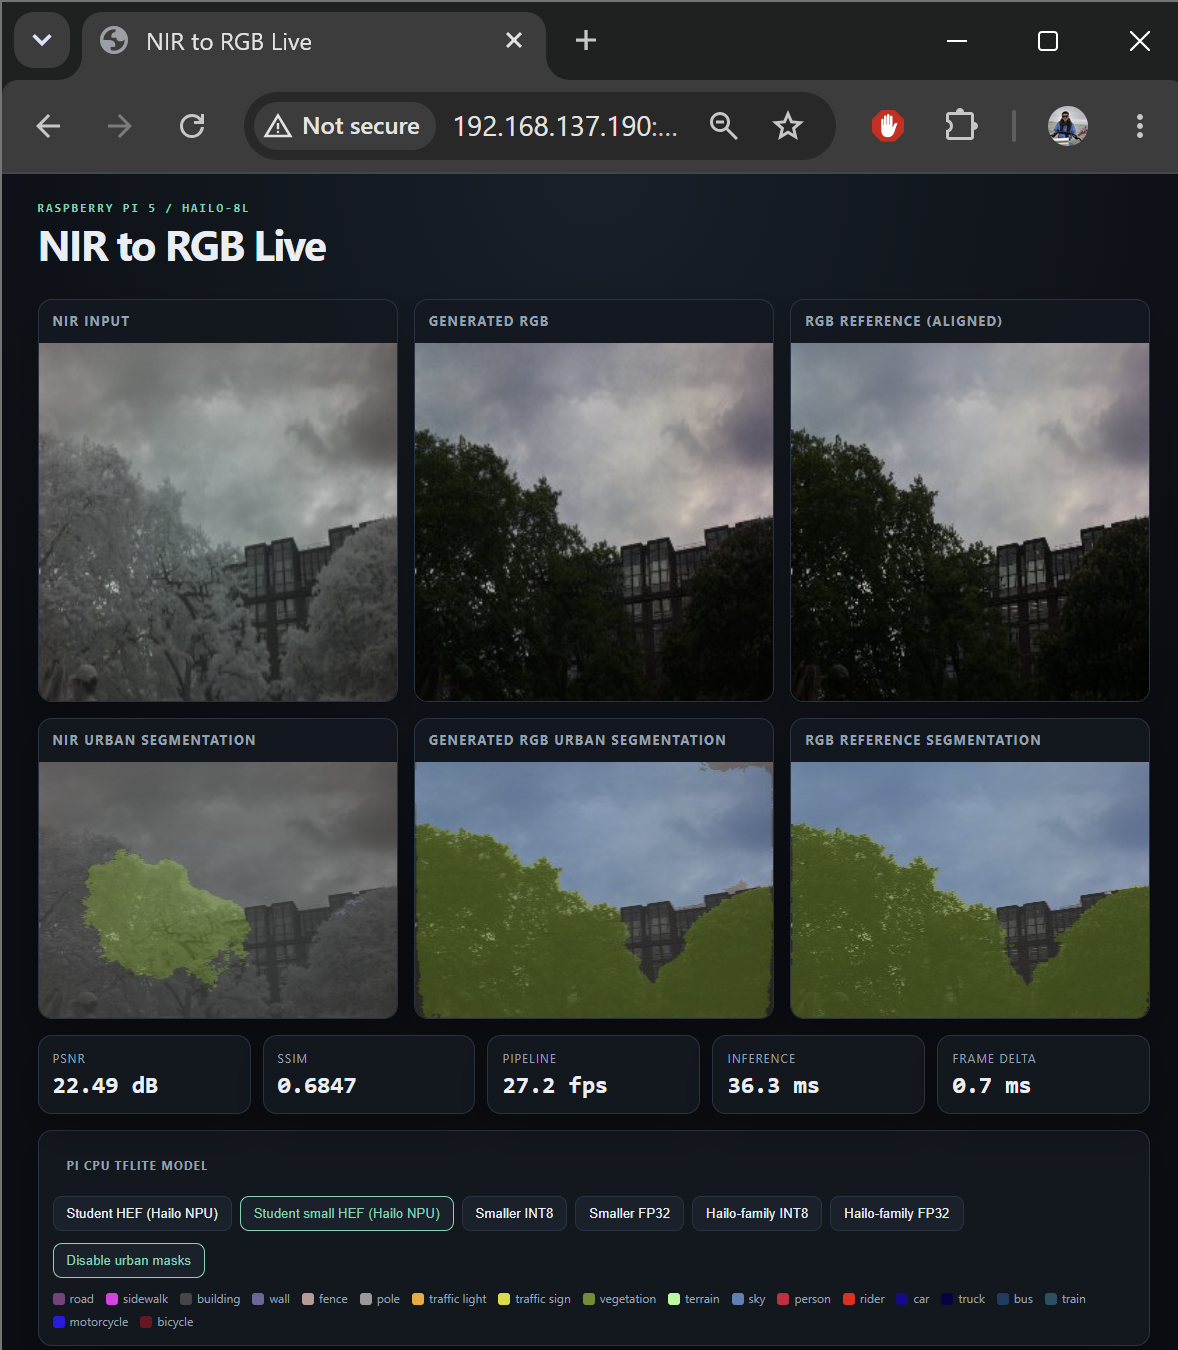
\includegraphics[width=\textwidth]{imgs/webapp_live_demo.png}
\caption{Live on-device web app demonstration on the Raspberry~Pi~5.}
\label{fig:webapp_live}
\end{figure}

\section{Robustness}
\label{sec:res_robustness}

The controlled robustness protocol of Section~\ref{sec:test_robustness} applies deterministic perturbations to the NIR input only, using the first 200 images of the canonical seed-42 test split without further shuffling. \autoref{tab:res_robustness} reports the paired change in each metric relative to the same model's unperturbed run on the same subset, for the final teacher and the selected FP32 student. 

\begin{table}[!htbp]
\centering
\scriptsize
\setlength{\tabcolsep}{3pt}
\resizebox{\linewidth}{!}{%
\begin{tabular}{llcccccccc}
\hline
 & & \multicolumn{4}{c}{\textbf{Teacher}} & \multicolumn{4}{c}{\textbf{Student FP32}} \\
\textbf{Perturbation} & \textbf{Level} & \textbf{$\Delta$PSNR (dB)} & \textbf{$\Delta$LPIPS} & \textbf{$\Delta$CLIP-B/16} & \textbf{$\Delta$DINOv2-L} & \textbf{$\Delta$PSNR (dB)} & \textbf{$\Delta$LPIPS} & \textbf{$\Delta$CLIP-B/16} & \textbf{$\Delta$DINOv2-L} \\
\hline
Exposure gain & 0.8 & -0.57 & +0.006 & -0.001 & -0.002 & -0.73 & +0.007 & -0.003 & -0.002 \\
Exposure gain & 1.2 & -0.74 & +0.002 & -0.002 & -0.003 & -1.14 & +0.005 & -0.002 & -0.005 \\
Gamma & 0.8 & -0.04 & +0.001 & 0.000 & 0.000 & -0.10 & +0.001 & 0.000 & 0.000 \\
Gamma & 1.2 & +0.01 & 0.000 & +0.001 & -0.001 & +0.01 & +0.001 & -0.001 & -0.002 \\
Gaussian blur & $\sigma=1$ & -3.07 & +0.209 & -0.042 & -0.079 & -3.61 & +0.239 & -0.050 & -0.113 \\
Gaussian blur & $\sigma=2$ & -8.47 & +0.509 & -0.179 & -0.367 & -6.75 & +0.499 & -0.144 & -0.300 \\
Gaussian noise & $\sigma=0.01$ & -0.73 & +0.026 & -0.017 & -0.022 & -1.37 & +0.045 & -0.015 & -0.038 \\
Gaussian noise & $\sigma=0.03$ & -5.66 & +0.208 & -0.085 & -0.159 & -5.58 & +0.236 & -0.095 & -0.154 \\
\hline
\end{tabular}
}
\caption{Robustness sweep on the first 200 images of the canonical test split. Each cell is the paired change relative to the same model's clean run on the same subset. Negative $\Delta$PSNR and $\Delta$cosine and positive $\Delta$LPIPS are degradations. Perturbations are applied to the NIR input only. Raw results are in \texttt{experiments/robustness\_v1/per\_image.csv}.}
\label{tab:res_robustness}
\end{table}

Exposure and gamma variation in the tested range is handled well, with the worst case across both models a 1.14\,dB PSNR loss and every embedding change at most 0.005 cosine. Blur and noise define the boundary of the operating envelope. At $\sigma=1$ blur and $\sigma=0.01$ noise the degradation is measurable but moderate, while at $\sigma=2$ blur the teacher loses 8.47\,dB PSNR and 0.367 DINOv2-L cosine and the student loses 6.75\,dB and 0.300, with noise at $\sigma=0.03$ close behind. At that blur level the perturbed outputs sit at DINOv2-L cosines near 0.55--0.57, below the raw-NIR full-test level of 0.728, so outside the envelope the translation no longer offers an embedding-agreement advantage over the untranslated input. These tests are diagnostic rather than a separate success criterion, supporting deployment where input sharpness and noise can be monitored and degraded frames rejected, not unconditional acceptance of arbitrary field conditions.

\section{Key Findings}
\label{sec:res_summary}

The results across this chapter support five main conclusions.

\begin{enumerate}
    \item \textbf{Downstream agreement, not pixel fidelity, is the criterion that matters.} Pix2Pix matches the student on PSNR and SSIM yet recovers almost none of the downstream behaviour, sitting at raw-NIR level on the independent DINOv2-L and depth probes. Pixel metrics alone would have ranked it as competitive and missed this.
    \item \textbf{The foundation-feature teacher closes most of the gap}, moving detection, segmentation, depth and independent embeddings substantially toward native-RGB behaviour, and the No-FM ablation confirms the feature ensemble drives these gains.
    \item \textbf{Distillation preserves that behaviour at a fraction of the size.} The 1.7\,M student keeps positive closure on all five primary tasks, a $67.3\times$ reduction from the teacher, and mixed-INT8 quantisation keeps every closure positive.
    \item \textbf{The student is the only edge-deployable model in the comparison}, meeting the 5\,FPS target on the Pi CPU and reaching 27.2\,FPS on the Hailo-8L NPU with no thermal throttling, while Pix2Pix at 54.4\,M parameters is far too large to run interactively on the device.
    \item \textbf{The recipe generalises only where there is spectral structure}, transferring to thermal but breaking down on SAR, which marks the boundary of the approach.
\end{enumerate}
